\documentclass{article}
\newcommand{\BEAS}{\begin{eqnarray*}}
\newcommand{\EEAS}{\end{eqnarray*}}
\newcommand{\BEQ}{\begin{equation}}
\newcommand{\EEQ}{\end{equation}}
\newcommand{\BIT}{\begin{itemize}}
\newcommand{\EIT}{\end{itemize}}

\newcommand{\eg}{{\it e.g.\ }}
\newcommand{\ie}{{\it i.e.\ }}

\newcommand{\ones}{\mathbf 1}
\newcommand{\zeros}{\mathbf 0}
\newcommand{\reals}{{\mbox{\bf R}}}
\newcommand{\integers}{{\mbox{\bf Z}}}
\newcommand{\symm}{{\mbox{\bf S}}}  % symmetric matrices

\newcommand{\nullspace}{{\mathcal N}}
\newcommand{\range}{{\mathcal R}}
\newcommand{\Rank}{\mathop{\bf Rank}}
\newcommand{\Tr}{\mathop{\bf Tr}}

\newcommand{\sign}[1]{\mathop{\textrm{sgn}}(#1)}
\newcommand{\lambdamax}{{\lambda_{\rm max}}}
\newcommand{\lambdamin}{\lambda_{\rm min}}

\newcommand{\EE}{\mathop{\textrm{E}}}
\newcommand{\Cov}{\mathop{\textrm{Cov}}}
\newcommand{\Prob}{\mathop{\bf Prob}}
\newcommand{\Co}{{\mathop {\bf Co}}} % convex hull
\newcommand{\dist}{\mathop{\bf dist{}}}
\newcommand{\argmin}{\mathop{\rm argmin}}
\newcommand{\argmax}{\mathop{\rm argmax}}
\newcommand{\epi}{\mathop{\bf epi}} % epigraph
\newcommand{\Vol}{\mathop{\bf vol}}
\newcommand{\dom}{\mathop{\bf dom}} % domain
\newcommand{\intr}{\mathop{\bf int}}


\newcommand{\nrm}[1]{\left\lVert#1\right\rVert}
\newcommand{\nrmo}[1]{\left\lVert#1\right\rVert_1}
\newcommand{\nrmt}[1]{\left\lVert#1\right\rVert_2}
\newcommand{\nrmnn}[1]{\left\lVert#1\right\rVert_{*}}
\newcommand{\nrmf}[1]{\left\lVert#1\right\rVert_F}

\newcommand{\myexp}[1]{\mathop{\rm exp}\left\{#1\right\}}
\newcommand{\mylog}[1]{\mathop{\rm log}\left\{#1\right\}}
\newcommand{\questions}{\begin{frame}Questions?\end{frame}}
\newcommand{\LL}{\textrm{LL}}
\newcommand{\KL}{\textrm{KL}}
\newcommand{\HH}{\textrm{H}}
\newcommand{\GG}{\textrm{G}}

\newcommand{\Bound}{\textrm{B}}
\newcommand{\bb}{\mathbf{b}}
\newcommand{\aaa}{\mathbf{a}}
\newcommand{\BB}{\mathbf{B}}
\newcommand{\AAA}{\mathbf{A}}
\newcommand{\CC}{\mathbf{C}}
\newcommand{\cc}{\mathbf{c}}
\newcommand{\mm}{\mathbf{m}}
\newcommand{\MM}{\mathbf{M}}
\newcommand{\nn}{\mathrm{\bf neighbors}}
\newcommand{\pa}[1]{{\textrm{\bf pa}}\left(#1\right)}
\newcommand{\pre}[2]{\mathop{\textrm{\bf pnp}}_{#1}\left(#2\right)}
\newcommand{\logsum}{\textrm{logsum}}

\newcommand{\tth}{{\textrm{th}}}
\newcommand{\xx}{\mathbf{x}}
\newcommand{\mmu}{\mathbf{\mu}}
\newcommand{\yy}{\mathbf{y}}
\newcommand{\zz}{\mathbf{z}}
\newcommand{\dd}{\mathbf{d}}
\newcommand{\new}{\textrm{new}}
\newcommand{\old}{\textrm{old}}
\newcommand{\fpr}{\textrm{FPR}}
\newcommand{\tpr}{\textrm{TPR}}
\newcommand{\auc}{\textrm{AUC}}
\newcommand{\yyi}{\yy_i}
\newcommand{\xxi}{\xx_i}
\newcommand{\vvec}[2]{\left[ \begin{array}{c} \mathbf{#1}\\ \mathbf{#2} \end{array}\right]}
\newcommand{\mmat}[4]{\left[ \begin{array}{cc} \mathbf{#1}&\mathbf{#2}\\ \mathbf{#3}&\mathbf{#4} \end{array}\right]}
\newcommand{\xyvec}{\left[ \begin{array}{c} \xx\\\yy \end{array} \right]}
\newcommand{\xyvecc}{\left[ \begin{array}{c} x^1\\y^1 \end{array} \right]}
\newcommand{\eye}{   \left[ \begin{array}{cc} 1 & 0 \\ 0 & 1 \end{array}\right]}
\newcommand{\bket}[2]{\left\langle#1,#2\right\rangle}
\newcommand{\bbket}[2]{\left\llangle#1,#2\right\rrangle}
\newcommand{\redq}{\textcolor{red}{q}}
\newcommand{\blup}{\textcolor{blue}{p}}
\newcommand{\BIEA}{\begin{IEEEeqnarray*}}
\newcommand{\EIEA}{\end{IEEEeqnarray*}}
\newcommand{\BIEAN}{\begin{IEEEeqnarray}}
\newcommand{\EIEAN}{\end{IEEEeqnarray}}
\newcommand{\pmin}{\mathop{\textrm{minimize}}}
\newcommand{\psubjto}{\textrm{subject to}}
\newcommand{\WW}{\mathbf{W}}
\newcommand{\ww}{\mathbf{w}}
\newcommand{\YY}{\mathbf{Y}}
\newcommand{\XX}{\mathbf{X}}
\newcommand{\UU}{\mathbf{U}}
\newcommand{\uu}{\mathbf{u}}
\newcommand{\VV}{\mathbf{V}}
\newcommand{\vv}{\mathbf{v}}
\newcommand{\PP}{\mathbf{P}}
\newcommand{\pp}{\mathbf{p}}
\newcommand{\rr}{\mathbf{r}}
\newcommand{\RR}{\mathbf{R}}
\newcommand{\ee}{\mathbf{e}}
\newcommand{\BA}{\mathbf{A}}

\newcommand{\aalpha}{{\boldsymbol\alpha}}
\newcommand{\llambda}{{\boldsymbol\lambda}}
\newcommand{\ddelta}{{\boldsymbol\delta}}
\newcommand{\otherwise}{\textrm{otherwise}}
\newcommand{\answer}{\fbox{\tt answer} }
\newcommand{\abs}[1]{\left| #1 \right|}

\newcounter{problemCtr}
\newcommand{\newproblem}[1]{\hrule\paragraph{Problem \theproblemCtr (#1)}\stepcounter{problemCtr}}


\newcounter{HW}

\usepackage{amsthm}
\usepackage{graphicx}
\usepackage{natbib}
\usepackage{algorithm}
\usepackage{algorithmic}
\usepackage{amsmath}
\usepackage{hyperref}


\newtheorem{remark}{Remark}
\newtheorem{lemma}{Lemma}
\newtheorem{definition}{Definition}
\newtheorem{proposition}{Proposition}
\newtheorem{assumption}{Assumption}
\newtheorem{corollary}{Corollary}
\newtheorem{theorem}{Theorem}


\usepackage{slashbox}
\setcounter{HW}{1}
\begin{document}

\author{Calvin Deutschbein}
\title{COMP  790-125, HW\theHW}
\maketitle



\newproblem{0.01pt} Open \texttt{hw\theHW.tex}, replace ``Wile E. Coyote'' with your name. Run
\texttt{pdflatex hw\theHW.tex}, look at hw\theHW.pdf, and confirm that your name is in the right place.


\newproblem{0.5pt}
\begin{enumerate}
\item Plot the sigmoid function in MATLAB using script
\begin{verbatim}
z = [-5:0.1:5];
fz = 1./(1 + exp(-z));
plot(z,fz,'LineWidth',3);
xlabel('z');ylabel('f(z)'); % we always label axes, yes we do!
hwplotprep
print -dpdf sigmoid.pdf
\end{verbatim}
Find the resulting figure in file {\tt sigmoid.pdf}.
\item In hw\theHW.tex, find the segment of the file that sets up the first figure -- it starts with {\tt \textbackslash begin\{figure\}} and ends with  {\tt \textbackslash end\{figure\}}. Inside this segment  replace {\tt emptiness.pdf} with {\tt sigmoid.pdf}.
\item Change the text under {\tt \textbackslash caption} -- right now it says ``This is emptiness, it earns no points.'' -- to say what the figure is about.
\item Remake hw\theHW.pdf by running in shell/command prompt

     \texttt{pdflatex hw\theHW.tex}

and check that your plot and caption are now in.
\end{enumerate}


\begin{figure}[H]
\begin{center}
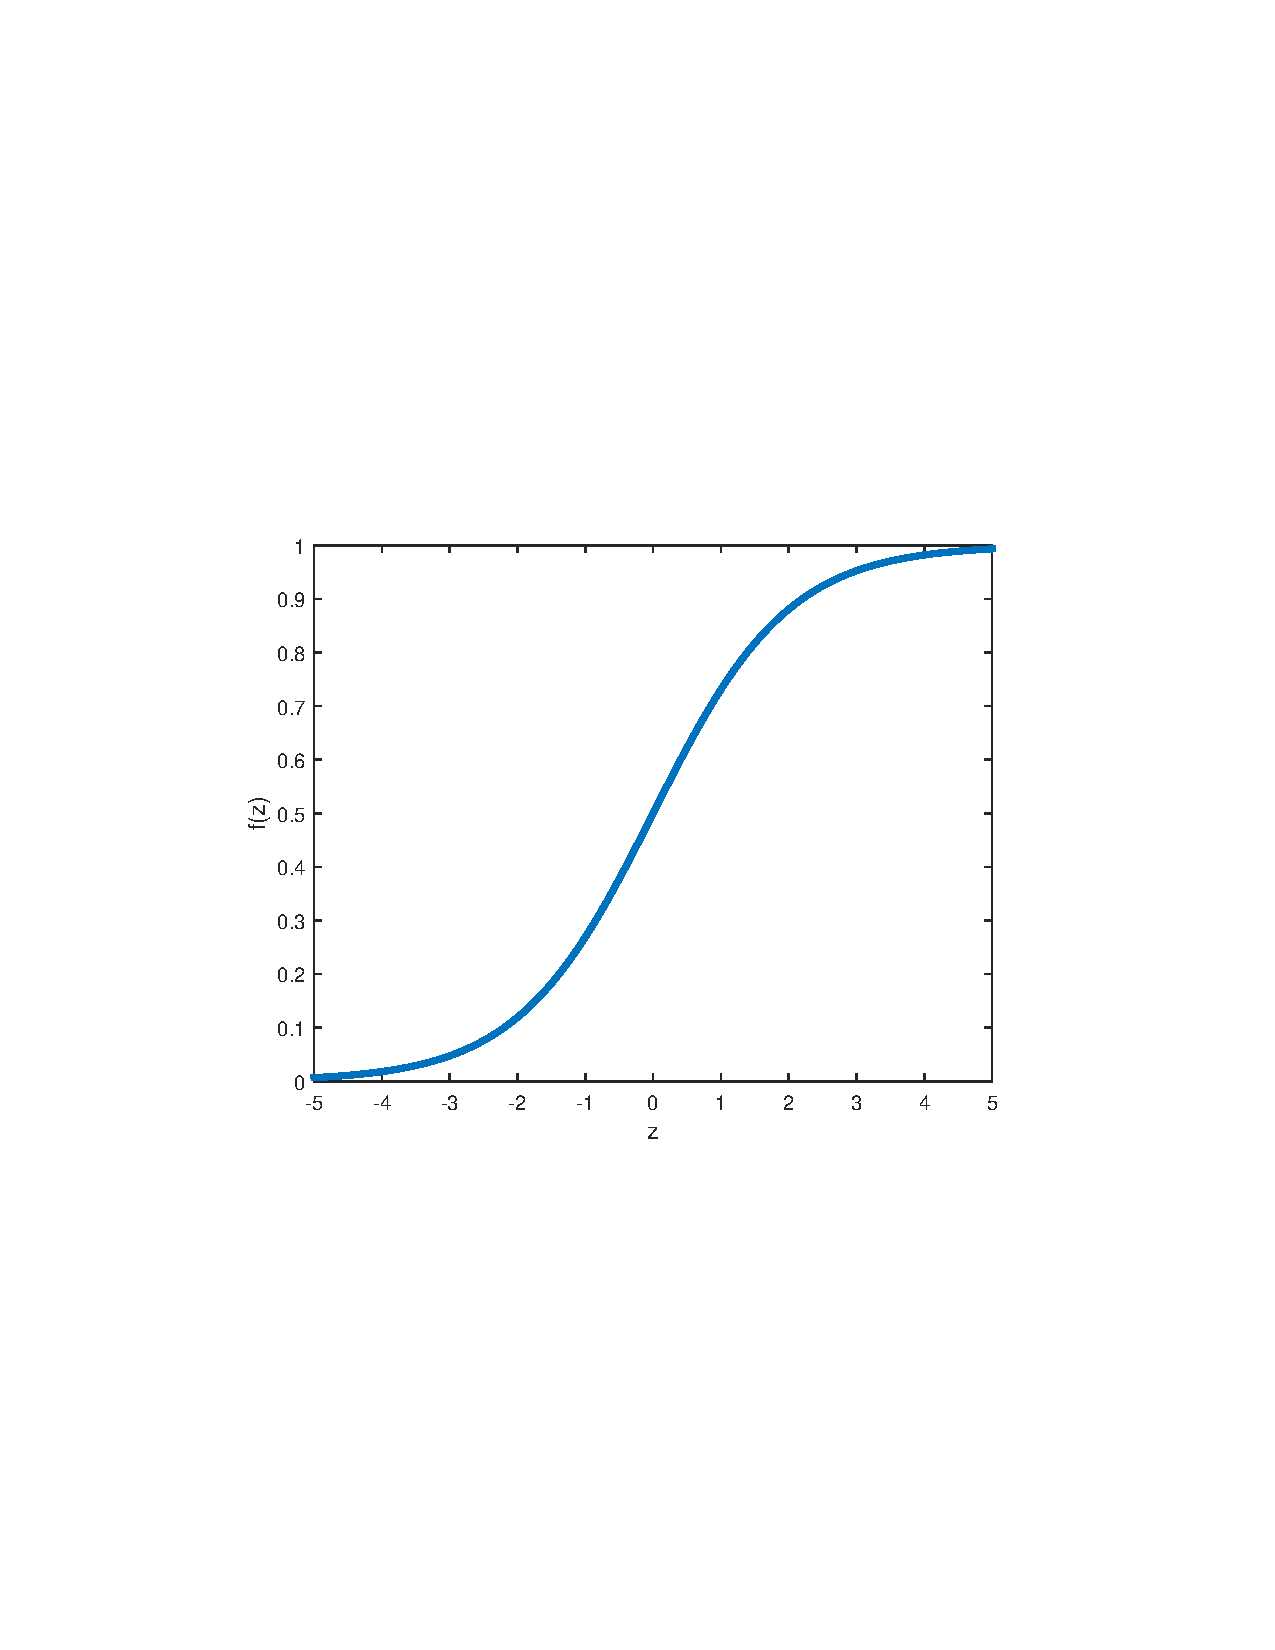
\includegraphics[scale=0.5]{sigmoid.pdf}
\caption{This is a sigmoid function.}
\end{center}
\end{figure}

\hrule

\newproblem{0.5pt}
Fill in the first derivative and second derivative of sigmoid function in the hw\theHW.tex.

The first derivative and second derivative
\[
\frac{d f(z)}{dz} =  \frac{e^x}{(e^x + 1)^2}, 
\frac{d^2 f(z)}{dz} =  \frac{-1}{(e^x + 1)}+\frac{3}{(e^x+1)^2}-\frac{2}{(e^x+1)^3}.
\]

\newproblem{0.5pt}
Write a MATLAB function that implements computation  of the first derivative of $f$ at a particular point. You just did the math for this.
Here is a function that is {\em wrong}
\begin{verbatim}
function d = dsigmoid(z)
% This function computes first derivative of sigmoid function at z
d = exp(x)/(exp(x) + 1)^2
end
\end{verbatim}

Created a file {\tt dsigmoid.m} that {\em correctly} computes the first derivative.

\newproblem{0.5pt}

We will use your function {\tt dsigmoid.m} to plot the first derivative.
\begin{verbatim}
zs = [-5:0.01:5];
for i = 1:length(zs)
    ds(i) = dsigmoid(zs(i));
end
plot(zs,ds,'LineWidth',3);
xlabel('z');ylabel('df(z)');
hwplotprep
print -dpdf dsigmoid.pdf
\end{verbatim}

Find the resulting plot in file {\tt dsigmoid.pdf}. In hw\theHW.tex replace {\tt emptiness.pdf} with {\tt dsigmoid.pdf} . Change the
caption in the figure to say what the figure is about. Remake hw\theHW.pdf and check that your plot has made it in.
\begin{figure}[H]
\begin{center}
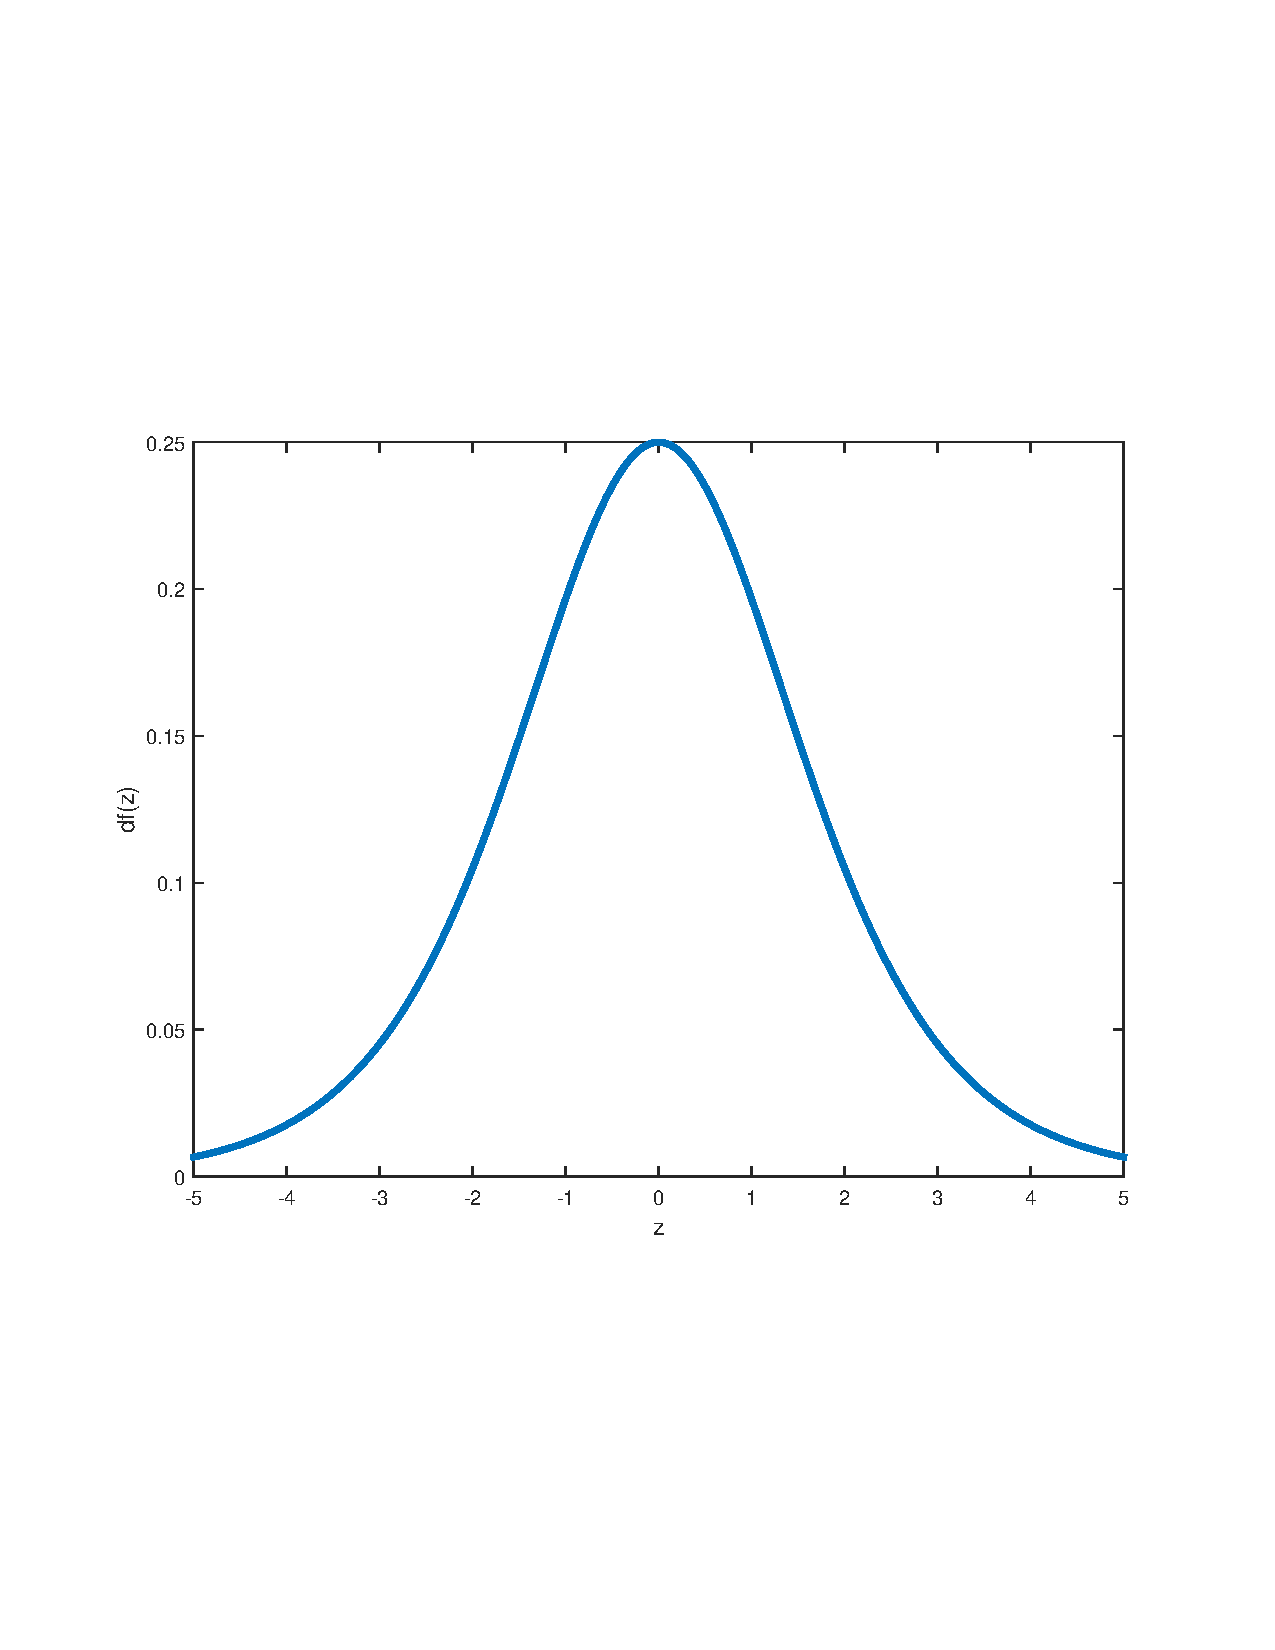
\includegraphics[scale=0.5]{dsigmoid.pdf}
\caption{This is dsigmoid.}
\end{center}
\end{figure}


\newproblem{0.5pt}
We can approximate derivatives numerically
\[
\frac{df(z)}{dz}\approx \frac{f(z+h) - f(z)}{h}
\]
where the right-side of this approximate equality is called {\em finite difference} approximation. Unlike derivative definition we do not need $h$ to be infinitesimal, just a small value. The numerical approximation of a derivative is tremendously useful trick to check you derivative, gradients, Jacobians, Hessians etc. Make sure that you understand what it does.

We will use this approximation to check your derivatives. Here is a function that computes approximately the derivatives of sigmoid
\begin{verbatim}
function d = fdsigmoid(z)
f0 = 1/(1 + exp(-z));
f1 = 1/(1 + exp(-(z + 1e-5)));
d = (f1 - f0)/1e-5;
end
\end{verbatim}
Save this function into a file names \texttt{fdsigmoid.m}.

Try following code in MATLAB
\begin{verbatim}
zs = randn(100,1);
for i=1:length(zs)
    err(i) = dsigmoid(zs(i)) - fdsigmoid(zs(i));
end
hist(err,30)
hwplotprep
print -dpdf hist.pdf
\end{verbatim}
The code above samples 100 normally distributed values and computes the finite differences approximation and the derivative you derived and implemented and then plots histogram of errors.

Find the resulting plot in file {\tt hist.pdf}. In hw\theHW.tex replace {\tt emptiness.pdf} with {\tt hist.pdf} . Change the
caption in the figure to say what the figure is about. Remake hw\theHW.pdf and check that your plot has made it in.
\begin{figure}[H]
\begin{center}
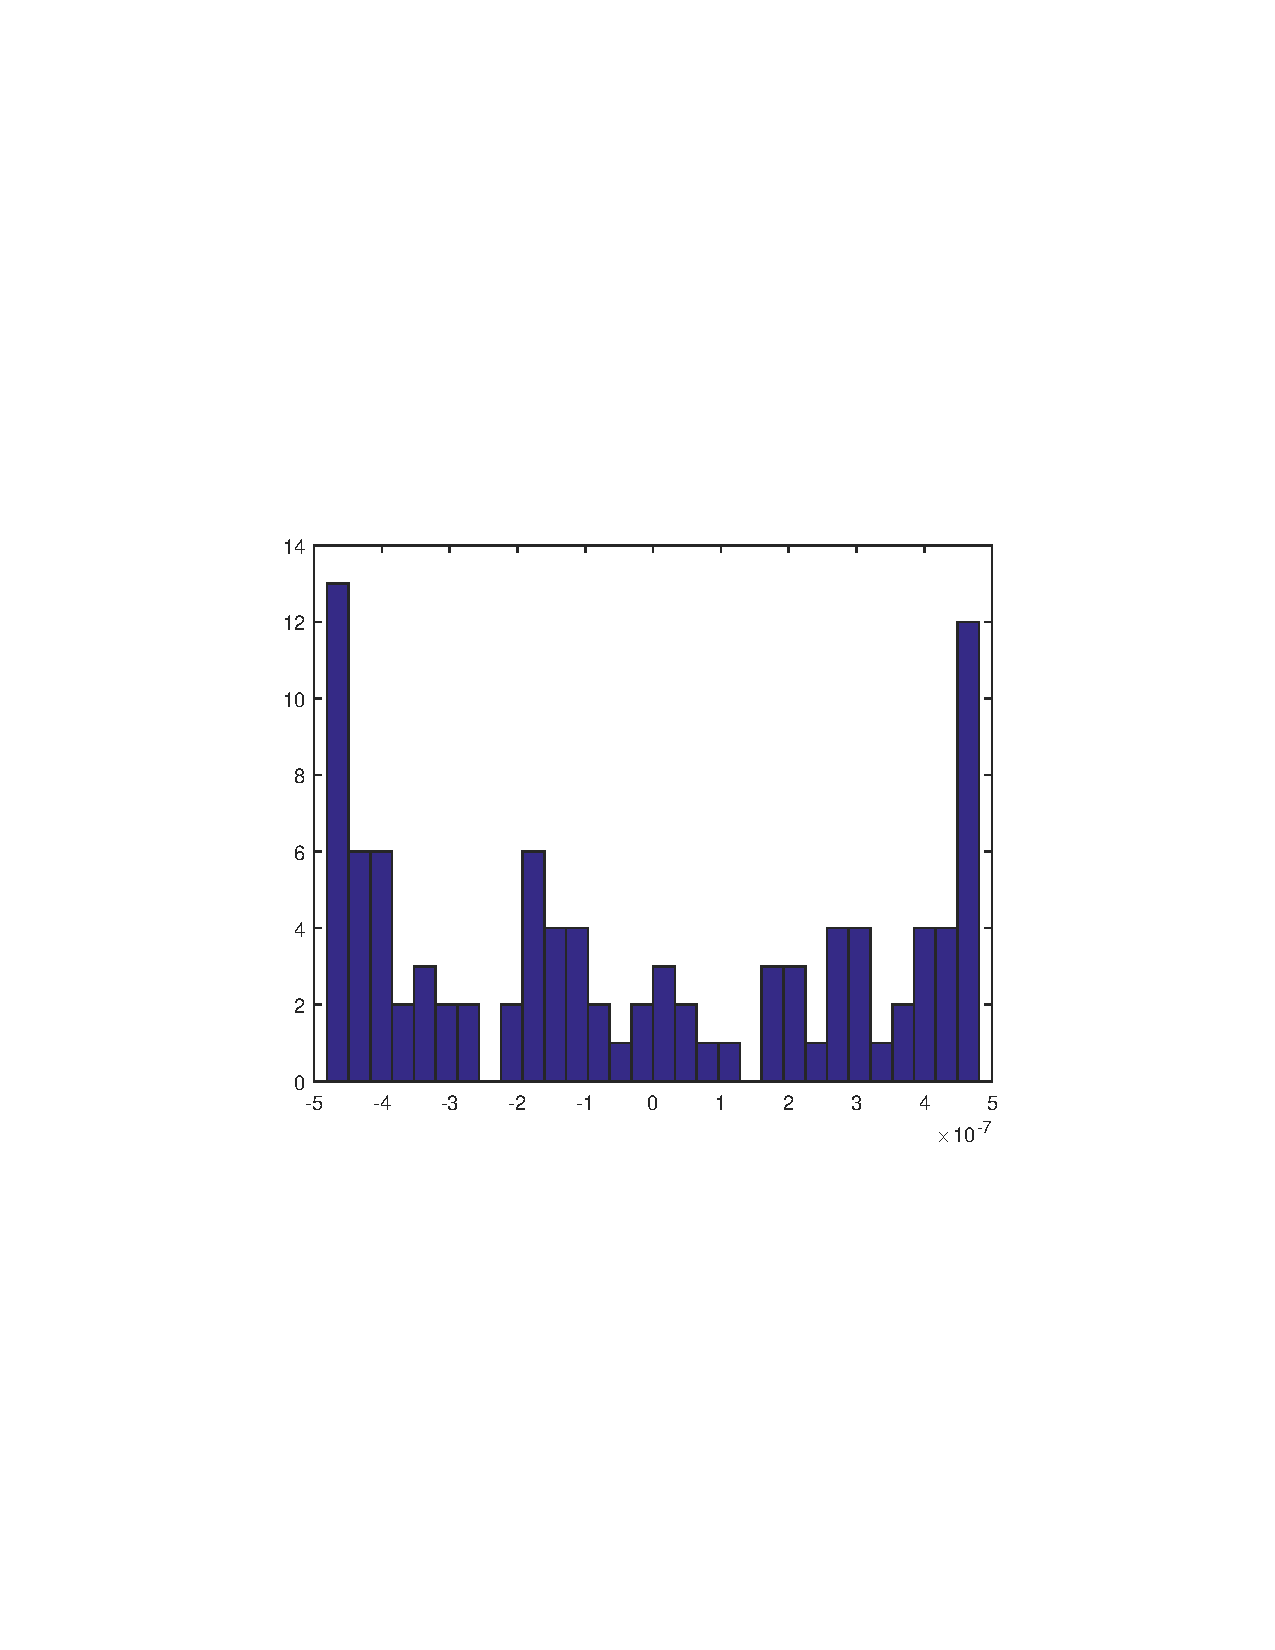
\includegraphics[scale=0.5]{hist.pdf}
\caption{This is the histogram.}
\end{center}
\end{figure}



\begin{remark} The error ranges between 0 and 13.
\end{remark}


\newproblem{0.5pt}
Let
\BEQ\label{eq:pz}
f(z) = \frac{1}{1 + \myexp{-z}} = p
\EEQ
express $z$ in terms of $p$
\[
z =  log(\frac{-p}{p-1}).
\]
Now suppose
\BEQ\label{eq:qz}
\frac{\myexp{-z}}{1 + \myexp{-z}} = q
\EEQ
and express $z$ in terms of $q$
\[
z =  log(\frac{1-q}{q}).  % log(\frac{1-q}{q}
\]
Given Eqs.\eqref{eq:pz},\eqref{eq:qz} express $q$ in terms of $p$
\[
q = pe^\frac{p}{p-1}.
\]
Express $f(-z)$ in terms of $f(z)$
\[
f(-z) = \frac{1}{1+e^z}.
\]
Hint: the manipulations that are useful here are either subtraction from 1 (as in $1-x$), computing inverse (as in $\frac{1}{x}$), and taking logarithm (as in $\log(x)$).

\section*{Log of sigmoid}
\newproblem{0.5pt}
Let $g(z)$ be log of sigmoid function
\[
g(z) = \mylog{ \frac{1}{1+ \myexp{-z}} }.
\]
Compute its derivative and fill it in here
\[
\frac{dg(z)}{dz} =  \frac{1}{1+e^z}.%1/(1+e^x)
\]
Check your derivative by comparing its value to the finite difference approximation.


\newproblem{0.5pt}
Compute second derivative of $g(z)$
\[
\frac{d^2g(z)}{d^2z} =  -\frac{e^x}{(1+e^x)^2}.%-e^x/(1+e^x)^2
\]
Check the second derivative by comparing its value to the finite difference of the {\em first} derivatives you computed above.

%I have 4/10 points at this point.


\newproblem{0.5pt}
Let the dataset be specified by $\mathcal{D} = \left\{ (\xx_i,y_i):i=1,\dots,n \right\}$. We specify conditional probability of $y$
\BEQ \label{eq:plr}
p(y_i | \xx_i,\beta_0,\beta) = \frac{1}{1 + \myexp{-y_i(\beta_0 + \bket{\beta}{\xx_i})}}
\EEQ
Write a matlab function that computes log probability of label $y$ given a vector of features $\xx$ and $\beta_0,\beta$.
\begin{verbatim}
function logP = logProbLogReg(y,x,beta0,beta)
logP =log(1/(1+exp(-y*(beta0+dot(beta,x)))))
end
\end{verbatim}
Now write a matlab function that uses the above function to compute log probability of label $+1$ for a vector of features $\xx$ and $\beta_0,\beta$
\begin{verbatim}
function predY = predictY(x,beta0,beta)
logProbY = logP(1,x,beta0,beta);
if logProbY > 0
    predY = 1
else
    predY = -1
end
\end{verbatim}
Hint: Since $p(y=1|x) + p(y=-1|x) = 1$, what is the threshold $p(y=1|x)$ has to exceed for you to predict that $y$ is 1? Consequently what is the threshold
that $\log p(y=1|x)$  has to exceed for you to predict that $y$ is 1?

Generalize this code so that it works for a matrix $\texttt{X}$ with each row being a sample, and returns predicted label for each sample.
\begin{verbatim}
function predY = predictY(X,beta0,beta)
C = num2cell(X,2)
cellfun(@(x) helppredY(x,beta0,beta), C)
end

function helppredY = helppredictY(x,beta0,beta)
logProbY = logP(1,x,beta0,beta);
if logProbY > 0
    helppredY = 1
else
    helppredY = -1
end
\end{verbatim}

\newproblem{0.5pt}
Given Eq.\eqref{eq:plr} we can write out log-likelihood
\BEQ \label{eq:ll}
\textrm{ALL}(\beta_0,\beta;\mathcal{D}) = \frac{1}{N}\sum_{i=1}^N \log \frac{1}{1 + \myexp{-y_i(\beta_0 + \bket{\beta}{\xx_i})}}.
\EEQ
Now using function $\texttt{logProbLogReg}$ that you obtained for the previous problem, write a matlab function that computes loglikelihood
\begin{verbatim}
function val = AverageLogLikLogReg(y,X,beta0,beta)
val = 0;
for i=1:length(y)
   val = val + (logP(y(i),X(i,:),beta0,beta) / length(y))
end
\end{verbatim}

%5/10

\newproblem{0.5pt}
Write a function that computes gradient of log-likelihood of logistic regression Eq.\eqref{eq:ll}
\begin{verbatim}
function [dbeta0,dbeta] = dAverageLogLikLogReg(y,X,beta0,beta)
h = 1e-5;
dbeta0 = (ALLLR(y,X,beta0+h,beta) - ALLLR(y,X,beta0,beta))/h;
for i=1:length(beta)
    f0 = ALLLR(y,X,beta0,beta);
    beta(i) = beta(i) + h;
    f1 = ALLLR(y,X,beta0,beta);
    beta(i) = beta(i) - h;
	dbeta(i) = (f1-f0)/h
end
end
\end{verbatim}
You can make sure that your implementation is correct using the finite differences trick.
\newproblem{0.5pt}
We will add ridge penalty term to log-likelihood

\BEQ \label{eq:pll}
\textrm{ALL}(\beta_0,\beta;\mathcal{D}) = \left(\frac{1}{N}\sum_{i=1}^N \log \frac{1}{1 + \myexp{-y_i(\beta_0 + \bket{\beta}{\xx_i})}}\right) + \lambda\sum_{j=1}^p \beta_j^2.
\EEQ

Note that ridge penalty does {\em not} apply to $\beta_0$.

Change functions {\texttt AverageLogLikLogReg} and {\texttt dAverageLogLikLogReg} so that they compute penalized average-log-likelihood, and its gradient, respectively.

\begin{verbatim}
function val = AverageLogLikLogReg(y,X,beta0,beta,lambda)
val = 0;
for i=1:length(y)
   val = val + (logP(y(i),X(i,:),beta0,beta) / length(y))
end
for i=1:length(beta)
    val = val + lambda * beta(i) * beta(i)
end
end

function [dbeta0,dbeta] = dAverageLogLikLogReg(y,X,beta0,beta,lambda)
h = 1e-5;
dbeta0 = (ALLLR(y,X,beta0+h,beta,lambda) - ALLLR(y,X,beta0,beta,lambda))/h;
for i=1:length(beta)
    f0 = ALLLR(y,X,beta0,beta,lambda);
    beta(i) = beta(i) + h;
    f1 = ALLLR(y,X,beta0,beta,lambda);
    beta(i) = beta(i) - h;
	dbeta(i) = (f1-f0)/h
end
end
\end{verbatim}
You can use finite differences to check the gradient.

%6/10

\newproblem{2pt}
Implement a gradient ascent algorithm for fitting logistic regression and paste it below.
Remember, gradient ascent iterates updates to parameters by taking a step in the direction of the gradient.  
\begin{verbatim}
function [beta0,beta] = fitLogReg(trainY,trainX,lambda,s)
beta0 = trainY(1)
beta = trainX(1,:)
for i=1:20
    [dbeta0,dbeta] = dgradient(trainY,trainX,beta0,beta,lambda);
    beta0 = dbeta0*s+beta0;
    beta = dbeta*s+beta;
end
end
\end{verbatim}

%8/10


\newproblem{1pt} In Matlab load data stored in \texttt{hw\theHW.mat}. There are six variables stored in this environment:
\texttt{trainX,trainy,validX,validy,testX,testy}. First two variables store a training set, second two a validation set, and the last two a test set.
You will inspect the dataset. 

Visualize sample $i$'s features by running 
\begin{verbatim}
imagesc(reshape(trainX(i,:),[192 168]));colormap(gray)
\end{verbatim}

What is the range of values in each sample's feature vector (\texttt{trainX(i,:)})? [0,255]

How many different label values are in the set (look at \texttt{trainy})? 2

What is the nature of the data? It is a multidimensional image.

\newproblem{2pt}
You will fit penalized logistic regression using the code you developed earlier. You will run this code for different combinations of step-sizes ( $10^{-1}$, $10^{-2}$, $10^{-3}$, $10^{-4}$, $10^{-5}$) and for penalty weight \texttt{lambda} ($0.001$, $0.01$, $0.1$, $0.2$, $0.4$, $0.8$, $1$) on the data stored in \texttt{hw\theHW.mat}.

Recall that \texttt{load hw\theHW.mat} loads the \texttt{trainy} and \texttt{trainX} variables.
You can train on this dataset by running command
\begin{verbatim}
[beta0,beta] = fitLogReg(trainy,trainX,lambda,s) 
\end{verbatim}

Write code that runs this fitting procedure for each step-size and $\lambda$ pair and stores resulting \texttt{beta0} and \texttt{beta}.
\begin{verbatim}
stepsizes = 10.^[-1 -2 -3 -4 -5];
lambdas = [0.001 0.01 0.1 0.2 0.4 0.8 1.0];
for i=1:length(stepsizes)
    for j=1:length(lambdas)
        [beta0s(i*length(lambas)+j),betas(i*length(lambas)+j)] = fitLogReg(trainy,trainX,lambdas(j),stepsizes(i));
    end
end
\end{verbatim}
This will amount to running the fitting procedure 35 times and getting new \texttt{beta0} and \texttt{beta} each time. 


Using stored \texttt{beta0} and \texttt{beta}, make predictions on validation set \texttt{validX} and compare the predicted labels to \texttt{validy}. 
If a predicted label differs from the corresponding value in \texttt{validy}, that sample has been misclassified. Misclassification error is the fraction of misclassified samples in 
the set. For example, if there are 10 misclassification errors on a set of size 135, then the misclassification error will be $\frac{10}{135} = 0.0741$.

On the validation set, compute misclassification error for each of the 35 stored \texttt{beta0} and \texttt{beta}. 

\begin{verbatim}
for i=1:length(stepsizes)
    for j=1:length(lambdas)
        val = 0;
        ind = i + length(lambdas)*j
        for k=1:length(validy)
            val = val + abs(validy(k)-predY(validX(k,:),beta0s(ind),betas(ind,:)));
        err(i,j) = val / length(validy);
    end
end
\end{verbatim}
Populate the table below with these errors. 

Matlab took it's sweet time here so I took the liberty of continuing on to latter sections and doing my best as I have some concern that it will complete in any reasonable amount of time at all.  I, unfortunately, am not experienced enough with matlab to be able to determine what aspects of my code are causing these high complexities.  I would welcome feedback in this area.


\begin{center}
\begin{tabular}{|c|c|c|c|c|c|c|c|}
\hline
\backslashbox{\texttt{s}}{\texttt{lambda}}&0.001&0.01&0.1&0.2&0.4&0.8&1 \\\hline
$10^{-1}$ &&&&&&&\\\hline
$10^{-2}$ &&&&&&&\\\hline
$10^{-3}$ &&&&&&&\\\hline
$10^{-4}$ &&&&&&&\\\hline
$10^{-5}$ &&&&&&&\\\hline
\end{tabular}
\end{center}
\newproblem{1pt}
Given the above validation errors, select the \texttt{beta0} and \texttt{beta} that achieve lowest misclassification error on the validation set.

For the selected \texttt{beta0} and \texttt{beta}, evaluate misclassification error on the test set, \texttt{testX} and \texttt{testy}. Report the \texttt{beta0}. 

Unfortunately, whatever trap I fell into in Matlab has also crippled my ability to answer this question with actual values.
\begin{verbatim}
beta0 = ...
\end{verbatim}
Sort the entries in \texttt{beta} based on their absolute value and the top 10 entries' indices.
\begin{verbatim}
indices_top10 = ...
\end{verbatim}
Report test set misclassification error.
\begin{verbatim}
testerr = ...
\end{verbatim}
\newproblem{2pt}
$\beta$ vector contains weights of entries in a feature vector. Hence, you can determine which features are more important than others by comparing their weights.
You already identified top 10 features based on their weights.
Explain which features are useful for correctly predicting the label, and why. 
Argue strengths and weaknesses of the dominant features.

Features are a single data value known across all samples for which the likelihood of a specific label being applied can be reasonably assumed.  The beta value on the features determines the strength or importance of the correlation of a certain feature with a label.

Features are useful when they have higher correlations.  However, a member of a set of features may not be useful despite having high meaningful correlations if it lacks independence from other features in a set such that by removing that feature and expressing it in terms of other features little information may be lost.  The value of a future is directly proportionate to the absolute value of its correlation with labels in proportion with its independence.

\end{document}
